%\VignetteEngine{knitr::knitr}
%\VignetteIndexEntry{SCnorm_vigette}
\documentclass{article}
%\usepackage{fullpage}
\usepackage{graphicx, graphics, epsfig,setspace,amsmath, amsthm}
%\usepackage{hyperref}
\usepackage{natbib}
%\usepackage{listings}
\usepackage{moreverb}

\RequirePackage{/Library/Frameworks/R.framework/Versions/3.3/Resources/library/BiocStyle/resources/tex/Bioconductor}

\AtBeginDocument{\bibliographystyle{/Library/Frameworks/R.framework/Versions/3.3/Resources/library/BiocStyle/resources/tex/unsrturl}}  
\usepackage{Sweave}
\begin{document}
\Sconcordance{concordance:SCnorm.tex:SCnorm.Rnw:%
1 9 1 1 2 1 0 1 2 1 1 1 0 17 1 1 2 1 0 1 2 1 0 1 1 3 0 1 2 1 1 1 2 4 0 1 2 12 1 %
1 2 1 0 1 1 9 0 1 2 4 1 1 2 1 0 1 1 6 0 1 2 10 1 1 3 5 0 1 2 8 1 1 4 2 0 1 4 6 0 %
1 3 7 1 1 2 1 0 2 1 1 2 4 0 1 2 7 1 1 3 1 0 2 1 1 2 5 0 1 3 17 1 1 2 1 0 1 2 1 0 %
1 1 3 0 1 2 38 1 1 3 2 0 1 3 4 0 1 2 3 1 1 3 5 0 1 2 6 1 1 3 2 0 1 3 4 0 1 2 5 1 %
1 2 24 0 1 2 7 1}

% \SweaveOpts{concordance=TRUE}
\title{SCnorm: a quantile-regression based approach for robust normalization of single-cell RNA-seq data}
\author{Rhonda Bacher and Christina Kendziorski}
\maketitle
\tableofcontents
\setcounter{tocdepth}{2}

\section{Introduction}
\label{sec:intro}
SCnorm (as detailed in Bacher* and Chu* {\it et al.}, {\it{submitted}}) 
is a quantile-regression based approach for robust normalization of 
single-cell RNA-seq data. SCnorm groups genes based on their count-depth relationship then applies a quantile regression to each group in order to estimate scaling factors which will remove the effect of sequencing depth from the counts. 

\section{Run SCnorm}
\label{sec:quickstart}
Before analysis can proceed, the SCnorm package must be installed.
\begin{Schunk}
\begin{Sinput}
> install.packages('SCnorm_x.x.x.tar.gz', repos=NULL, type="source")
\end{Sinput}
\end{Schunk}

After successful installation, the package must be loaded into the working space:
\begin{Schunk}
\begin{Sinput}
>   library(SCnorm)
\end{Sinput}
\end{Schunk}
  
  \subsection{Required inputs}
\label{sec:startgenedeinput}
\begin{flushleft}
{\bf Data}:  The matrix \verb+Data+ should be a $G-by-S$ matrix
containing the expression values for each gene and each cell,
where $G$ is the number of genes and $S$ is the number of cells/samples. The matrix should contain
estimates of gene expression. Counts of this nature may be obtained from RSEM, HTSeq, Cufflinks, Salmon or a similar approach.
\end{flushleft}

\noindent The object \verb+ExampleData+ is a simulated data matrix containing
5,000 rows of genes and 180 columns of cells. 

\begin{Schunk}
\begin{Sinput}
> data(ExampleData)
> str(ExampleData)
\end{Sinput}
\begin{Soutput}
 num [1:5000, 1:180] 3.81 21.7 2.13 22.68 0 ...
 - attr(*, "dimnames")=List of 2
  ..$ : chr [1:5000] "X_1" "X_2" "X_3" "X_4" ...
  ..$ : chr [1:180] "C1_1" "C1_2" "C1_3" "C1_4" ...
\end{Soutput}
\end{Schunk}
  
  Here we simulated data as in SIM 1 (as detailed in Bacher* and Chu* {\it et al.}, {\it{submitted}}) with K = 4 (four slope groups), each condition has 90 cells and condition 2 has been 
sequenced approximately 4 times as much as condition 1.

{\bf Conditions}: The object \verb+Conditions+ should be a vector of length $S$ indicating which condition each cell belongs to. The order of this vector should match the order of the columns in the \verb+Data+ matrix.
\begin{Schunk}
\begin{Sinput}
> Conditions = rep(c(1,2), each= 90)
> str(Conditions)
\end{Sinput}
\begin{Soutput}
 num [1:180] 1 1 1 1 1 1 1 1 1 1 ...
\end{Soutput}
\end{Schunk}
  
  
  
  \subsection{SCnorm: Check count-depth relationship}
\label{sec:checkData}
Before normalizing using SCnorm, it is advised to check the count-depth relationship in your data. If all genes have a similar relationship then a global strategy such as median-by-ratio in the DESeq package or TMM in edgeR will be adequate. However, in our paper we show that a count-depth relationship that varies among genes leads to poor normalization when using global scaling strategies, in which case we strongly recomend proceding with the normalization provided by SCnorm. 

The function below will estimate the count-depth relationship for all genes, genes are first divided into groups based on their non-zero median expression, then the density of slopes for each group is plot. We recomend checking a variety of filter options, in case you find that only genes expressed in very few cells or very low expressors are the main concern.

The evaluation plot will be saved as a PDF in the current directory with file name specified in OutputName, or the path and filename may be supplied in OutputName (e.g., OutputName = "Desktop/FavoriteData/check\_myData").

\begin{Schunk}
\begin{Sinput}
> checkCountDepth(Data = ExampleData, Conditions = Conditions, OutputName = "check_exampleData", 
+                 FilterCellProportion = .1)
\end{Sinput}
\end{Schunk}
  
\begin{figure}[h!]
\centering
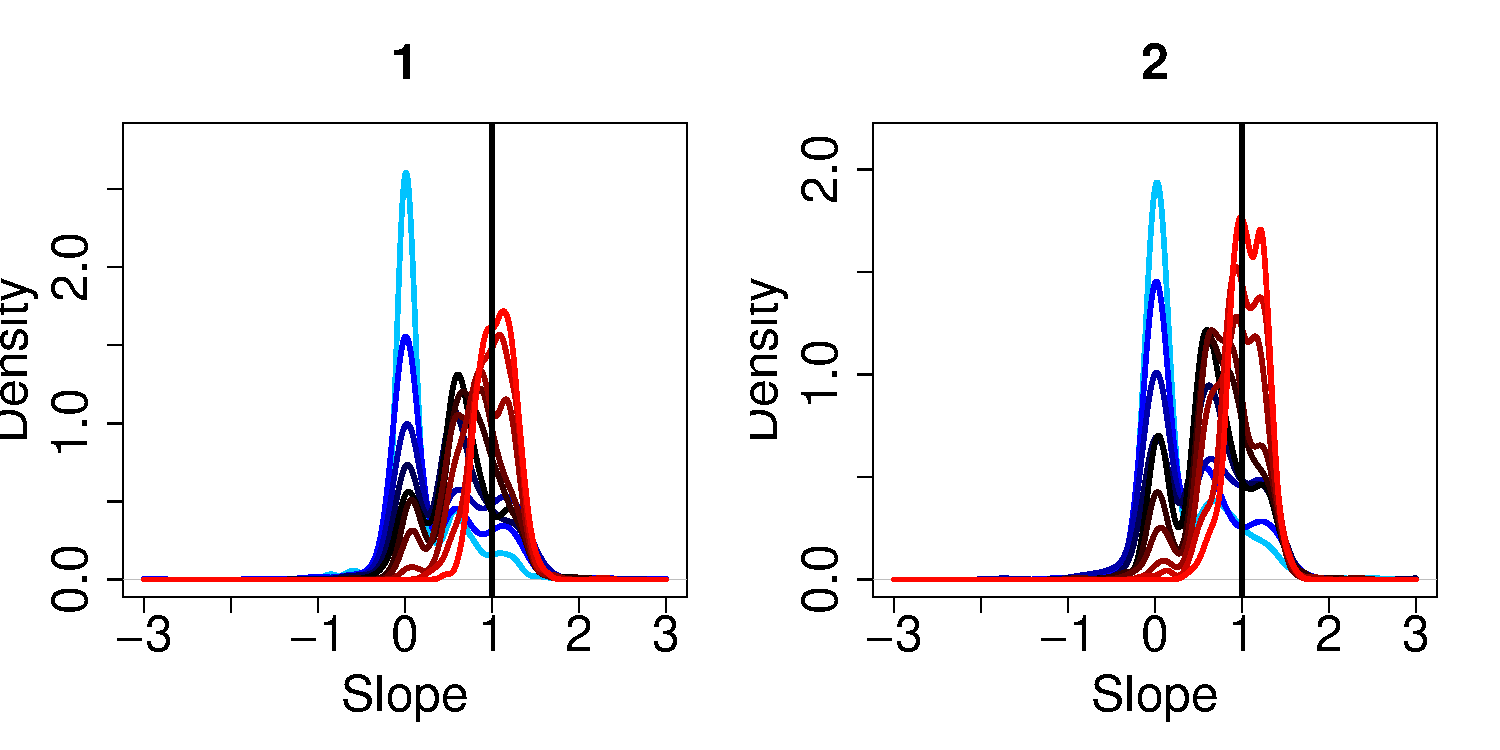
\includegraphics[width=.7\textwidth]{check_exampleData_initial_evaluation.pdf}
\caption{Evaluation of count-depth relationship in un-normalized data.}
\end{figure}

\newpage
It can also be used to evaluate data normalized by other methods:
\begin{Schunk}
\begin{Sinput}
> # Total Count normalization, Counts Per Million, CPM. 
> ExampleData.Norm <- t((t(ExampleData) / colSums(ExampleData)) * mean(colSums(ExampleData))) 
> checkCountDepth(Data = ExampleData, NormalizedData = ExampleData.Norm, 
+                 Condition = Conditions, OutputName = "check_exampleDataNorm",  
+                 FilterCellProportion = .1, FilterExpression = 2)
> 
\end{Sinput}
\end{Schunk}

\begin{figure}[h!]
\centering
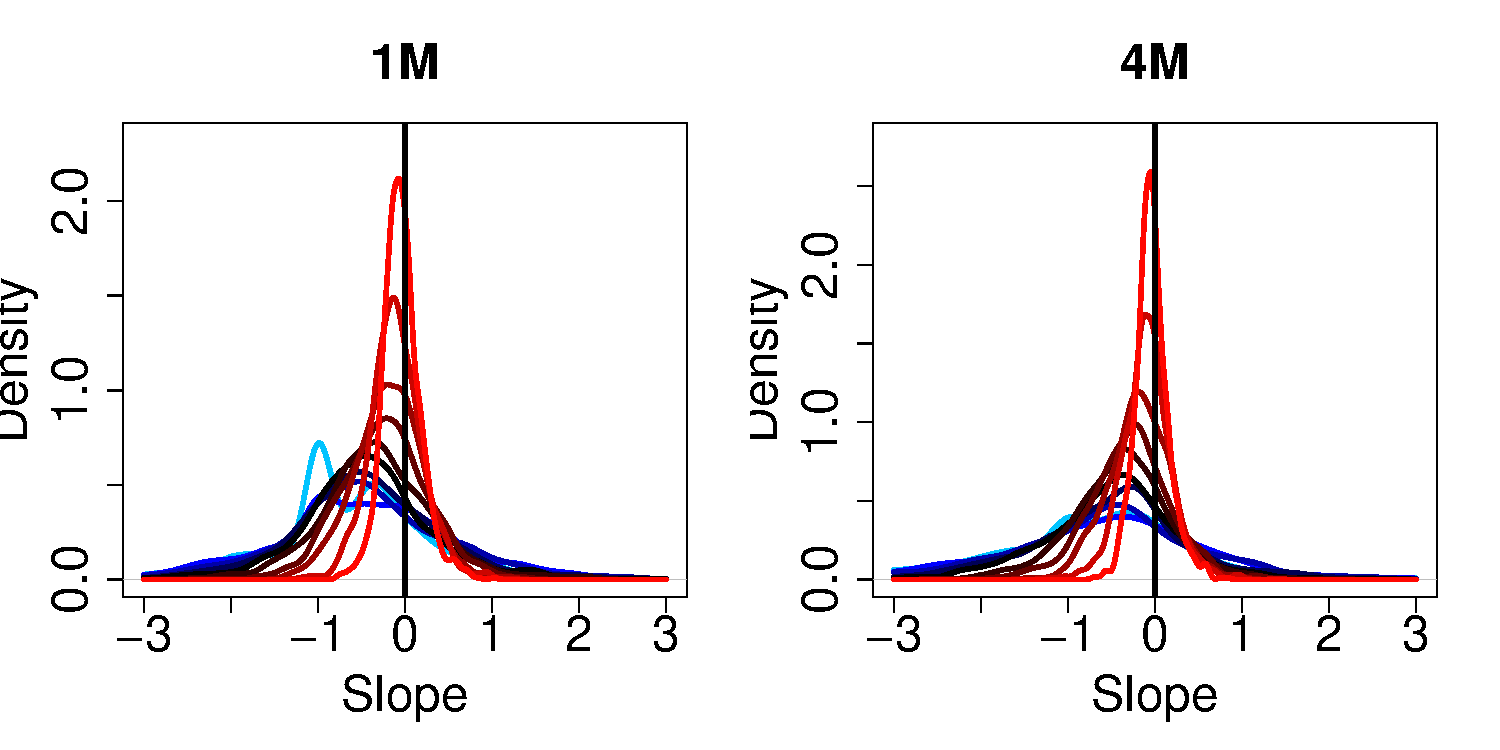
\includegraphics[width=.7\textwidth]{check_exampleDataNorm_count-depth_evaluation}
\caption{Evaluation of count-depth relationship in counts per million normalized example data.}
\end{figure}

Evaluating the bulk dataset included in the paper:
\begin{Schunk}
\begin{Sinput}
> library(SCnorm)
> data(bulkH1data)
> Conditions <- rep(1, dim(bulkH1data)[2])
> checkCountDepth(Data = bulkH1data, Condition = Conditions, OutputName = "check_bulkData", 
+                 FilterCellProportion = .1, FilterExpression = 2)
\end{Sinput}
\end{Schunk}

\begin{figure}[h!]
\centering
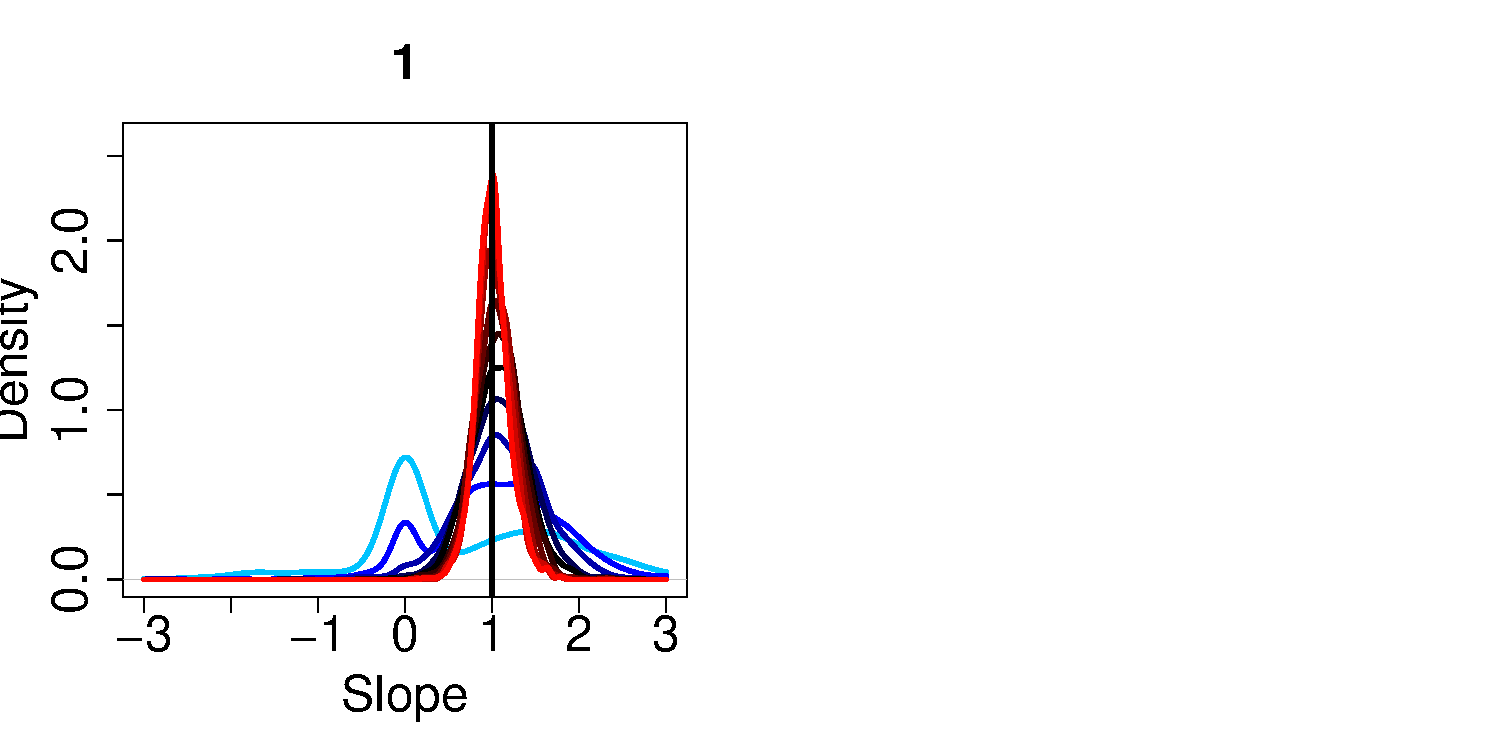
\includegraphics[width=.7\textwidth]{check_bulkData_initial_evaluation}
\caption{Evaluation of count-depth relationship in un-normalized bulk H1 data.}
\end{figure}

Evaluating the H1 single cell dataset included in the paper:
\begin{Schunk}
\begin{Sinput}
> library(SCnorm)
> data(scH1data)
> Conditions <- rep(c("1M", "4M"), each=92)
> checkCountDepth(Data = scH1data, Condition = Conditions, OutputName = "check_scData", 
+                 FilterCellProportion = .1, FilterExpression = 2)
> 
\end{Sinput}
\end{Schunk}

\begin{figure}[h!]
\centering
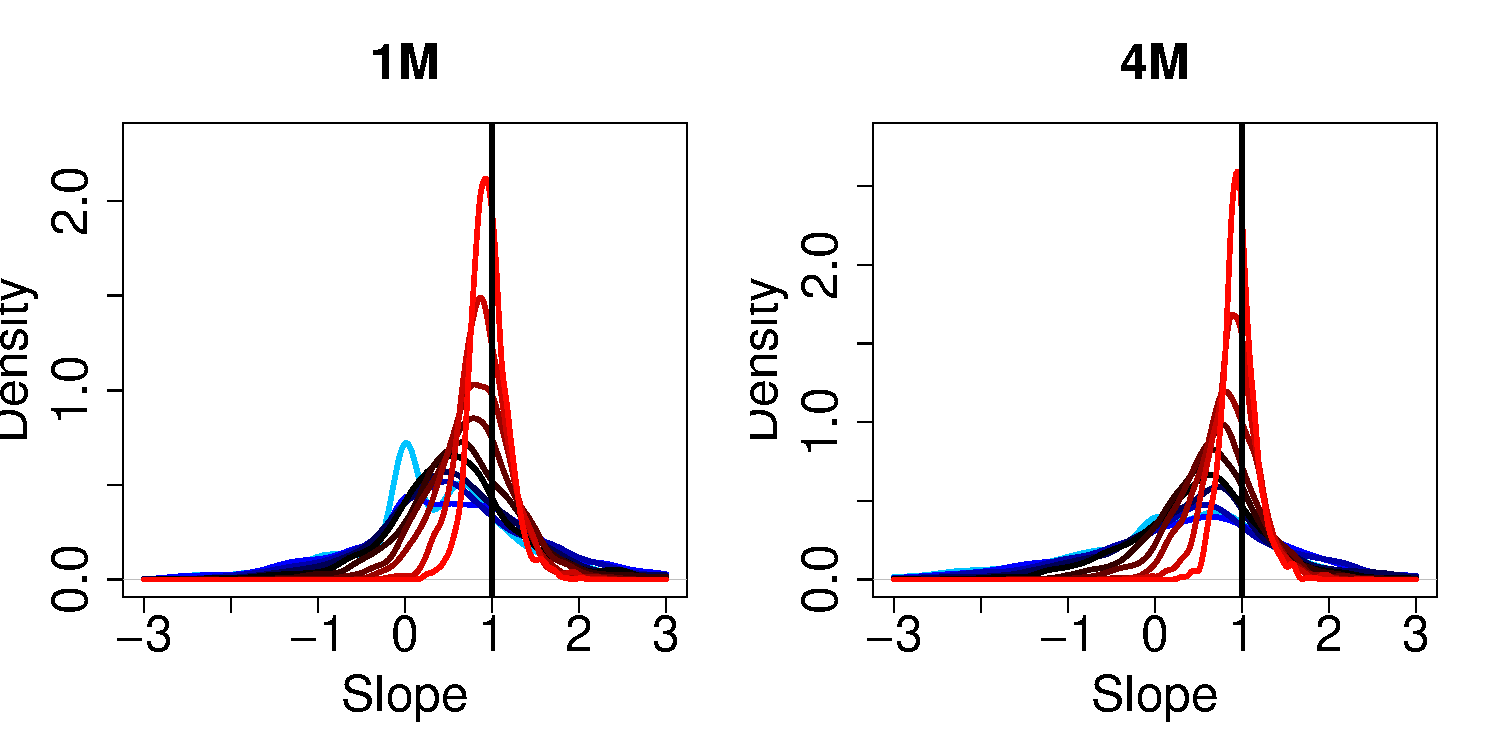
\includegraphics[width=.7\textwidth]{check_scData_initial_evaluation}
\caption{Evaluation of count-depth relationship in un-normalized H1 single cell data.}
\end{figure}




  \subsection{SCnorm: Normalization}
\label{sec:Normalization}
SCnorm will normalize across cells to remove the effect of sequencing depth on the counts and return the normalized expression counts, a list of genes which were not considered in the normalization due to filter options, and optionally an additional matrix of scale factors (default = FALSE).The default filter for SCnorm only considers genes having at least 10 non-zero expression value. The user may wish to adjust the filter and may do so by changing the value of FilterCellNum. Names of filtered genes are in DataNorm\$GenesFilteredOutGroupX, where X depends on the values in the Condition vector.

If PLOT=TRUE is specified, a plot of the progess of SCnorm will be created for each value of K tried.

Normalized data can be accessed by calling DataNorm\$NormalizedData.

\begin{Schunk}
\begin{Sinput}
> Conditions = rep(c(1,2), each= 90)
> DataNorm <- SCnorm(ExampleData, Conditions, OutputName = "MyNormalizedData",
+                      PLOT=TRUE, FilterCellNum = 10)
> str(DataNorm)
\end{Sinput}
\end{Schunk}
\begin{Soutput}
List of 3
 $ NormalizedData        : num [1:5000, 1:180] 9.55 47.44 5.34 56.88 0 ...
  ..- attr(*, "dimnames")=List of 2
  .. ..$ : chr [1:5000] "X_1" "X_2" "X_3" "X_4" ...
  .. ..$ : chr [1:180] "C1_1" "C1_2" "C1_3" "C1_4" ...
 $ GenesFilteredOutGroup1: chr(0) 
 $ GenesFilteredOutGroup2: chr(0) 
\end{Soutput}

\subsection{Evaluate choice of \textit{K}}
\label{sec:NormalizationK}

SCnorm first fits the model for $K = 1$, and sequentially increases K until a satisfactory stopping point is reached. For each value of $K$, SCnorm will estimate the count-depth relationship on the normalized counts. Gene evaluation groups are formed by splitting genes into 10 groups based on their non-zero median un-normalized expression and for each group the mode of the normalized count-depth relationship is estimated. If the absolute value of the maximum mode is < .1, then $K$ is selected, otherwise $K$ is increase by one.


\begin{figure}[h!]
\centering
\includegraphics[width=.5\textwidth]{MyNormalizedData_k_evaluation.pdf}
\caption{Evaluation of K}
\end{figure}



In Figure 5, $K = 4$ is chosen, once all 10 slope densities have absolute value of slope mode < .1.


\section{SCnorm: Multiple Conditions}
When more than one condition is present SCnorm will first normalize each condition independently then apply a scaling procedure between the conditions. In this step the assumption is that most genes are not differentially expressed (DE) between cells, that any systematic differences in expression across the majority of genes is due to technical bias and should be removed.

Generally the definition of condition will be obvious given the experimental setup. If the data are very heterogenous within an experimental setup it may be beneficial to first cluster more similar cells into groups and define these as conditions in SCnorm.

\section{SCnorm: UMI data}
SCnorm may also be applied to UMI data. It is highly recomended to check the count-depth relationship before and after normalization. In some cases, it might be desired to adjust the threshold used to decide K, the default value is .1. This means the largest slope mode must be within .1 of zero (zero indicates effective normalization), however lowering the threshold may improve results from some datasets. 

If the data have -many- ties (lower coverage UMI datasets), then the option ditherCounts should be set to TRUE (default is FALSE). This introduces some randomness but results will not change if the command is rerun.

For larger datasets, it may also be desired to increase the speed. One way to do this is to change the parameter PropToUse. PropToUse controls the proportion of genes to use for the group fitting, where the 25\% are chosen as those nearest to the the overall group mode. The default value is 25\%. 

\begin{Schunk}
\begin{Sinput}
> checkCountDepth(Data = umiData, Condition = Conditions, OutputName = "check_umi_scData", PLOT=TRUE,
+ FilterCellProportion = .1, FilterExpression = 2)
> DataNorm <- SCnorm(umiData, Conditions, OutputName = "MyNormalizedUMIData",
+ PLOT=TRUE, FilterCellNum = 10, PropToUse = .1, Thresh = .05, ditherCounts = TRUE)
\end{Sinput}
\end{Schunk}


\section{Session info}
Here is the output of sessionInfo on the system on which this document was compiled:
\begin{Schunk}
\begin{Sinput}
>   print(sessionInfo())
\end{Sinput}
\begin{Soutput}
R version 3.3.1 (2016-06-21)
Platform: x86_64-apple-darwin13.4.0 (64-bit)
Running under: OS X 10.11.6 (El Capitan)

locale:
[1] en_US.UTF-8/en_US.UTF-8/en_US.UTF-8/C/en_US.UTF-8/en_US.UTF-8

attached base packages:
[1] parallel  stats     graphics  grDevices utils     datasets  methods   base     

other attached packages:
[1] SCnorm_1.1.0   reshape2_1.4.2 moments_0.14   cluster_2.0.4  quantreg_5.29 
[6] SparseM_1.72  

loaded via a namespace (and not attached):
 [1] Rcpp_0.12.8        lattice_0.20-33    grid_3.3.1         plyr_1.8.4        
 [5] MatrixModels_0.4-1 magrittr_1.5       stringi_1.1.1      Matrix_1.2-6      
 [9] BiocStyle_2.1.33   tools_3.3.1        stringr_1.1.0     
\end{Soutput}
\end{Schunk}
  
  \vspace{1cm}
%\bibliographystyle{natbib}


%\bibliography{lengetal}

\end{document}
